\section{Implementation in an Existing Environment}\label{sec:challenges}

In the following section, we summarize the general setup of the TESS system at HCE (\cref{sec:hce_market_setup}), and describe how we position TESS in the existing tariff system (\cref{sec:position_tariff_system}) as well as our approach to designing device bidding functions (\cref{sec:HCE_design}), followed by the presentation of our financial settlement process (\cref{sec:hce_settlement}). We then describe the challenges associated with such a brownfield deployment (\cref{sec:impl_challenges}) and conclude with a description of planned extensions (\cref{sec:extensions}).

\subsection{General Setup}\label{sec:hce_market_setup}

In the HCE environment we use the technical setup of TESS as described in \cref{sec:technical_setup} to implement much of the standard design of the TS. All participating homes are represented by home hubs that bid on behalf of the customers \citep{powernet2021}. In terms of DER, we include photovoltaics, electric vehicle charging, and electric storage. Each participating device is further connected to a controller that can provide relevant physical information (such as current solar generation or the state-of-charge of electric storage) to the home hub for the purpose of bidding and implement the subsequent market allocation. Every five minutes, the home hubs send bids to the market operator. In addition, in the roles of the retailer and grid operator, HCE provides information on the supply cost, available import capacity, and unresponsive load. Bids are then cleared in a centralized double auction. 

The market result is characterized by an equilibrium price and the share of the marginal bid (`mode'). The latter equals 1 if the marginal bid (i.e. the bid(s) that determine the market price) can be fully cleared and is between 0 and 1 if that is not the case. For instance, if solar systems are generating more than can be exported, the bid will only partially clear and solar systems must reduce their generation to, for instance, 80\%.

Once, the market is cleared, home hubs compare their devices' bids to the equilibrium price. If the bid price exceeds the equilibrium price (for demand) or is less (for supply), the bid was cleared. 
If price and bid are equal, the bid was marginal and might be only partially cleared, corresponding to the share of the marginal bid.
This information is picked up by the device API and implemented physically, if possible.

All agents are implemented on the cloud and values (measurements, bids, market results) are stored in the TESS database, for validation and billing purposes.

\subsection{Positioning TESS in the Current Tariff System}\label{sec:position_tariff_system}

As HCE is a member-owned electric cooperative, they do not require approval by the relevant utility commission to change and adjust their tariffs. However, the management is responsible to their members and, in general, any substantial tariff changes increase the complexity of the underlying process, including metering, accounting, and billing. 

In some previous TS designs, participants were subscribed to a distinct transactive tariff (e.g. \citet{Widergren2014}).
We think, however, that a well-designed integration of the TS into the existing tariff system facilitates the deployment of TS in real-world settings. Specifically, we propose to leverage HCE's existing tariff Distribution Flexibility Program (DFP). Under the current design of the DFP, customers grant control over their DER to HCE and, in return, receive a bill credit. This bill credit is based on the type and number of DER included into the program and their performance. TESS would replace the current mechanism of controlling DERs and determining the applicable bill credit: instead of the current HCE control, DER dispatch would now be price-based, determined through the TS. Also, the applicable bill credit would be based on the payments received by the TS. As such, TESS could be seen as a specification of operating the Distribution Flexibility Program, fitting TESS neatly into the existing tariff system and avoiding the creation of new tariff categories.
Other tariffs, in particular the fixed retail rate and net metering, remain active, and DER owners can be on multiple rates simultaneously. 

We illustrate the stacking of tariffs with the following example. A customer pays a fixed retail rate on his electricity consumption during the billing period. 
If he also owns a solar panel (potentially procured through DERSA), he can additionally take advantage of net metering. Under net metering, the fixed retail rate only applies to his net consumption, i.e. the gross electricity consumption minus the electricity generated by the solar panel. 
Finally, the customer can opt in to participate in DFP. A bill credit would compensate the customer for any inconvenience from load curtailments or foregone payments from solar generation, if curtailed.

\subsection{Designing Bidding Functions in an Existing Tariff Structure}\label{sec:HCE_design}

Stacking multiple pre-existing retail rates for DER owners affects how customers participate in the TS. Here we present our design of a TS under the incentive structure imposed by the existing tariff regime as detailed in \cref{sec:HCE_tariff}. 
In previous TS implementations such as \citet{hammerstrom_2008}, the implementation of the TS disregarded the existing tariff system. As the system was fully integrated, customers were not able to opt out but received a side-payment that ensured that they did not experience any losses.

Two problems arise in the model of a closed system with side payment. 
First, while side payments are possible in an experimental context, they are a major obstacle to scaling up a TS in a broader implementation. 
Second, if outside options were not incorporated into bidding with an open system, the implemented bidding strategies would be sub-optimal for the customer, i.e. the system would not be incentive compatible, and customers would either override or leave the TS. Moreover, customers would switch to third parties such as load aggregators, which could then arbitrage between the existing tariff and the TS, resulting in a sub-optimal equilibrium.
Designing incentive-compatible bidding functions is therefore a crucial requirement to improve consumer welfare and open up the system to other stakeholders, such as manufacturers of smart home systems and devices or load aggregators.

To demonstrate the general approach of economic bidding with outside options, we focus on photovoltaics (PV).
Given net metering, any additional kWh generated decreases the customer's monthly bill $C$ by the retail rate $RR$.\footnote{Under net metering, the marginal value of export and the marginal value of consumption are identical and, under normal conditions, equal the fixed retail rate.} The cost-minimizing customer therefore faces the following objective function,

\begin{align}
    \min_\mathbf{q} C &= (\sum_t q^d_t - \sum_t q^s_t) RR \\
    \& s.t. q^{PV}_t \leq \overline{q}^{PV}_t, \forall t \nonumber
\end{align}

To minimize the bill, the customer will therefore generally generate the maximum electricity $q^{PV}_t = \overline{q}^{PV}_t$ possible, which is exogenous given weather conditions and installed capacity.
While the customer cannot increase generation, the customer could, of course, disconnect the system or decrease infeed below the technical limit $q^{PV}_t < \overline{q}^{PV}_t$, but he does not have any incentive to do so as that would imply missing out on substantial bill reductions, as described earlier. 
Therefore, customers with solar panels follow the rationale to use and/or export any electricity that the panel is generating.

The customer can, however, provide flexibility within the DFP program by decreasing solar generation or increasing net load at the rate of current production and receive a dispatch-dependent flexibility payment for participation. In that case, the new cost function is defined as follows,

\begin{align}
    C^{DFP} &= (\sum_t q^d_t - \sum_t q^s_t) RR - B(\mathbf{q}).
\end{align}

Curtailment would result in an increase of the bill by the fixed retail rate for each kWh not generated because of the curtailment. However, the customer is willing to provide this flexibility if compensated for the loss, i.e. if,

\begin{align}
    \frac{d B(\mathbf{q}^{PV})}{d q^{PV}_t} > RR .
\end{align}

The combination of the PV technology behavior and the NEM rate describes the baseline against which the customer will evaluate any changes he makes to his behavior.
The individual participation constraint therefore requires the customer to receive at least the retail rate as a compensation. Therefore, the customer would place a bid in the TS to reduce supply (or increase net load) at the minimum price of the retail rate $RR$  (price bid).
The amount of possible flexibility would correspond to the current solar infeed $\overline{q}^{PV}_t$ because, at best, the customer could fully shut down his solar generation (quantity bid). Conversely, the customer is not able to offer any negative baseline reductions, i.e. increase solar generation. \cref{fig:lem_adjustment_normal} illustrates this baseline effect.
Given this bidding strategy, the customer would accumulate a bill credit $B(\mathbf{q})$ which compensates the customer for the losses experienced from solar curtailment.

\begin{figure}[t]\label{fig:baseline}
  \begin{subfigure}[t]{0.485\linewidth}
    \centering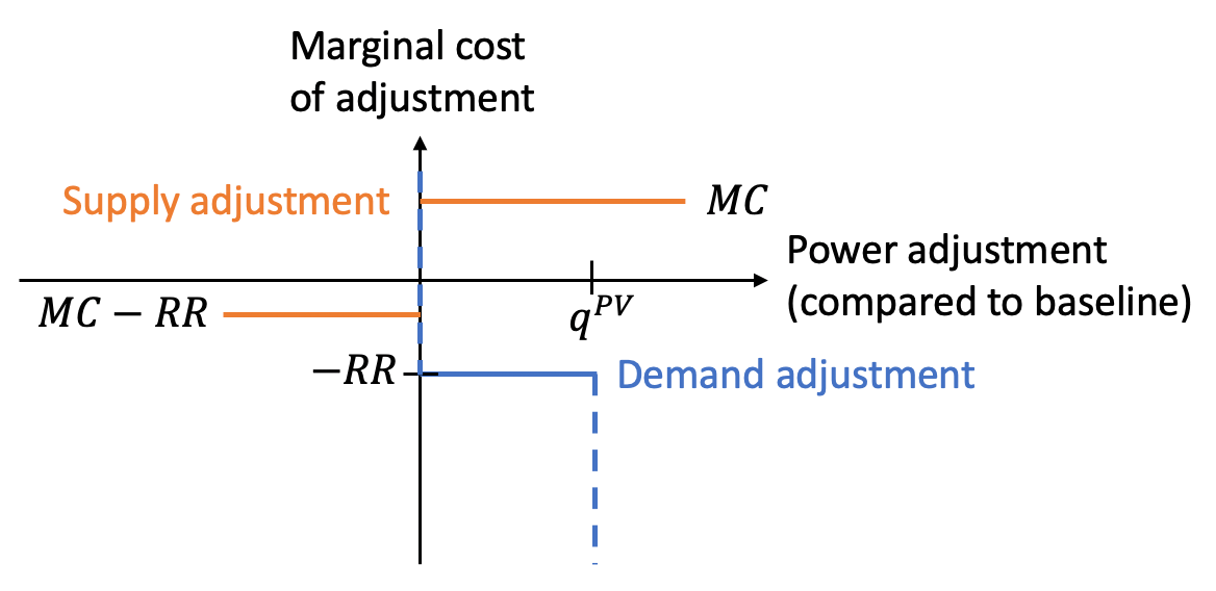
\includegraphics[height=3.2cm]{Market_power_normal_3.png}
    \caption{Market under normal supply conditions}
    \label{fig:lem_adjustment_normal}
  \end{subfigure}\hspace{0.5cm}
  \begin{subfigure}[t]{.485\linewidth}
    \centering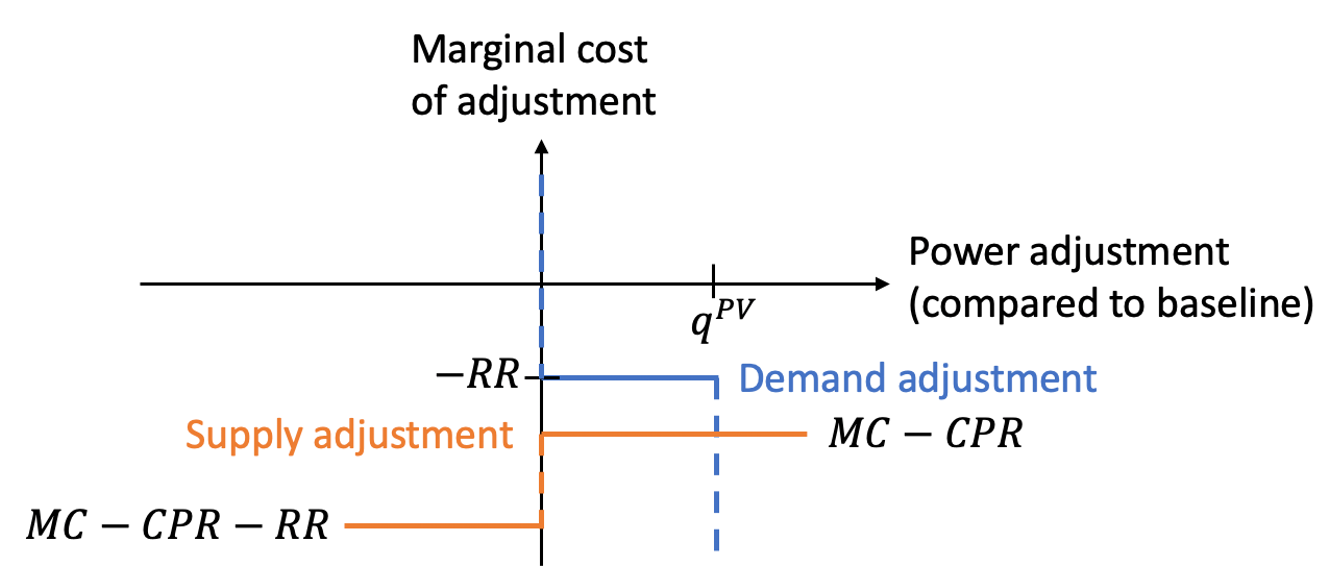
\includegraphics[height=3.2cm]{Market_power_adjustment_3.png}
    \caption{Market under requirement to increase net load} 
    \label{fig:lem_adjustment}
  \end{subfigure}
\caption{Market for power adjustment (compared to baseline)}
\end{figure}

We further analyze the bidding behavior of HCE. HCE is a cooperative and follows a complex combination of objectives, including commitments to resilience and energy supply sustainability. To derive the optimal bidding strategy, we abstract from that complexity and model HCE as a profit-maximizing entity, as many of those objectives are incorporated in their long-term investment and procurement decisions. Furthermore, with our focus on PV, this essentially translates into a cost-minimization problem. The decision variable is HCE's bidding strategy through which they can influence demand and supply participating in the TS,

\begin{align}
    \max \pi_\mathbf{b} &= \sum_t [\sum_{ij} (q^d_{ijt}(\mathbf{b}) -  q^s_{ijt}(\mathbf{b})) RR - MC_t q^{WS}_t + peak_t CPR_t |q^{WS}_t - \overline{q}^{WS}_t| ] + T(\mathbf{b}) \nonumber \\
    & s.t. \sum_{ij} q^d_{ijt}(\mathbf{b}) =  \sum_{ij} q^s_{ijt}(\mathbf{b}) + q^{WS}_t
\end{align}

The objective function includes income from net retail sales and the cost of energy procurement. The latter depend on the occurrence of a peak event, with $peak_t \in \{0;1\}$. Finally, the objective function includes the income of operating the transactive system. 

Under normal conditions ($peak_t = 0$), of course, HCE would not be willing to pay a customer the retail rate to reduce generation. Instead, it would sell additional generation at its long-term marginal supply cost $MC_t$ (and even take a price less than the fixed retail rate). On the other hand, it would be only willing to reduce supply from the baseline scenario if paid the foregone profit, i.e. the difference between the retail rate and the marginal cost. The bids provided by HCE and consumers are illustrated in \cref{fig:lem_adjustment_normal}. The curves do not intersect and the market allocation is empty.

A situation is possible, however, during which HCE would want to decrease generation within its distribution grid or, equivalently, increase net load to a level of $\overline{q}^{WS}_t$. Such a peak event ($peak_t = 1$) could arise when there is an abundance of renewable energy in the grid. Then, the entity operating the overlying grid could be willing to pay a critical peak rate $CPR$ to HCE for net load increases. Alternatively, HCE would need to curtail renewable energy within its system and pay them a compensation of $CPR$. In that case, the HCE bid changes and it would be willing to sell at a negative price, $MC_t - CPR$, i.e. pay consumers to consume more. Further decreasing supplies would be even more costly for the marginal unit, as HCE would miss out on sales at the fixed retail rate. 
The bids provided by HCE and consumers are illustrated in \cref{fig:lem_adjustment}. Now, supply and demand adjustments intersect at a quantity of $q^{PV}_t$ and the clearing price $p_t$ would be determined between $p \in [MC_t - CPR, -RR]$. Because the price is negative, the cash flow reverses and buyers get paid, while the seller pays.

Importantly, given the outside options of customers (in particular net metering), our design of the TS does not trade energy or power, but rather the deviation from this baseline generation or consumption. Thus the clearing price on the market reflects the price of \textbf{deviating} from the baseline. As a result, bids must reflect the quantity by which customers would be willing to deviate from the baseline and at what price. 

\cref{fig:pv_profile} illustrates the resulting implementation of the market result for a single customer with a solar system. For demonstration purposes, solar generation is approximated as a continuous normal distribution function. Generation starts in the early morning hours, reaches its maximum around noon, and terminates after sunset. The home hub, on behalf of the controller, continuously provides bids for increasing net load/reducing generation at the respective current generation $q^{PV}$, according to the described bidding strategy. Now assume that an adverse event occurs at 1pm, the market is cleared, and the solar system is shut down. In that case, solar generation is reduced to zero. In the subsequent market interval, no current (counterfactual) generation is available. For the implementation at HCE that relies on deviation from a baseline, we therefore approximate the available load reduction (i.e. to keep the solar system curtailed) using the most recent measurement. Therefore, the reduction for which the customer is eventually paid at settlement, corresponds to the red straight line of counterfactual generation during the adverse event. Once the situation dissolves, the market does not clear anymore and the solar system goes back online.

\begin{figure}[t]
\centering
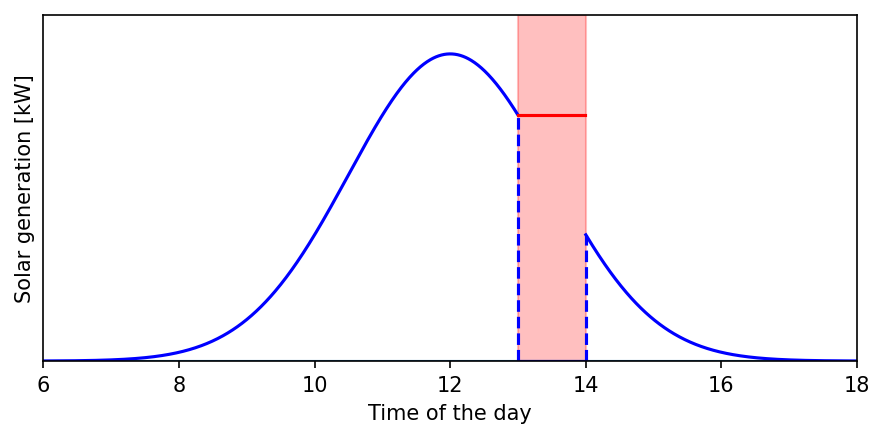
\includegraphics[scale=0.8]{TESS_PV_reduction.png}
\caption{PV curtailment}
\label{fig:pv_profile}
\end{figure}

TESS will integrate other DERs, specifically electric vehicle chargers and electric storage, at a later stage of the field deployment. Other device bidding functions will reflect the technical capabilities of each device and the opportunity costs and outside options of their owners. However, the baseline bidding strategies of PV panels as well as other DER come with significant challenges which will be discussed in \cref{sec:impl_challenges}.

\subsection{Settlement in TESS}\label{sec:hce_settlement}

In the last section, we described the bidding and market clearing in monetary terms, at given marginal costs and value. An additional problem in real-world systems, however, is that often actual costs/value only become clear in real-time or even  \textit{ex post}. One example is the cost of consuming or the value of producing during a coincident peak event. In the case of HCE, coincident  peak events happen at the time of the maximum net load in the Xcel system within a month. During the coincident peak, marginal consumption is significantly more expensive than during the rest of the month. However, it is unclear when it will actually happen within a month. For instance, overall load could be forecast to be very high during a day of the first week and the marginal supply costs would be supposedly very high, i.e. $MC_{coin} >> MC$. However, it might turn out that, later during the month, aggregate demand would be even higher. In that case, \textit{ex post}, the supply adjustment cost bid by HCE in the TS would have been wrong and any load adjustments would have been less valuable than previously thought. As a results, the bill credit required to be granted by HCE to responding customers would exceed the actual value they provided to the system.

Therefore, TESS will support tokens as a substitute for USD to bid in the TS. For a first implementation of our TS, we assume that customers have a prior of 1 token corresponding to the value of 1 USD. Therefore, any bids they make in USD could be translated into token bids on a 1:1 rate. 
At the end of the billing period, however, the market operator (here: HCE) would be able to calculate the total turnover of tokens during the month and determine the actual token value by comparing the turn-over to the savings achieved thanks to the operations of the TS. Multiplying the tokens collected by a customer with the final token value would give the final bill credit.

For the monthly bill of the customer, all tariffs need to be included again. The general electricity bill will be based on the read-out from the net meter, i.e. the net consumption during the billing period, multiplied by the fixed retail rate. In addition, TESS customers will be granted a bill credit, as foreseen in the DFP specification. Instead of a fixed amount per participating DER, the bill credit will depend on the turn-over of tokens the devices realized within TESS, multiplied by the value of a token. If, for instance, the solar panel of a customer disconnected due to an adverse event, the customer receives the product of the increase in net demand (equivalently, the reduction in generation) as compared to the base line, the token price paid by HCE for this deviation, and the token value in USD. As customers would not be willing to participate for a price below the fixed retail rate because of the net metering outside option, so their losses due to decreased solar generation will at least be off-set by the aggregate bill credit.

\subsection{Implementation Challenges}\label{sec:impl_challenges}

The implementation of TS in brownfield deployments comes with several challenges.
First, baseline approaches (i.e. providing demand flexibility as compared to a usual/expected load baseline) usually suffer from gaming. Customers could influence their baseline calculation to be able to report a bigger deviation from it and receive higher payments. In the case of PV, this risk is limited as HCE has access to the rated power of the system bidding as well as the PV measurements prior to the event. The latter can serve as a myopic forecast for the limited duration of a possible event requiring to increase net load. Moreover, HCE has access to data of solar panels that are not participating in TESS which provide a control baseline. Given these opportunities to validate customers' bids, we believe it is reasonable that customers bid their possible deviation to the best of their knowledge and specify the home hub to bid the latest measurement of PV generation as a possible deviation during the time when the system has not been curtailed. 
The problem becomes more severe, however, for other devices such as electric vehicles. It still needs to be determined how a baseline could be determined for other devices and whether information from such devices'  can be used to verify its bidding behavior.

Second, even if a baseline can be established, the baseline approach changes the distribution of surplus between the utility as well as customers with different devices. In the case of solar, customers will still enjoy the benefits of net-metering, even at times when the value of generation is far below the level of the fixed retail rate. Such effects can lead to inefficient investment in the long-term, as compared to a greenfield deployment with marginal value/cost bidding.

Third, the introduction of tokens opens up new opportunities, but also challenges. 
With regard to opportunities, tokens can be used to reimburse customers further for other beneficial actions, like the provision of data or energy efficiency investments. In theory, this compensation could be accomplished in USD, but other programs like Ohm Connect \citep{OhmConnect2020} and recent insights in gamification have shown that such tokens provide greater operational flexibility and might better be able to incentivize system-friendly behavior.
On the other hand, the introduction of tokens introduces another layer of uncertainty with regard to token value. Therefore, bidding should actually be based on the expected token value rather than on a fixed ``myopic'' assumption with respect to the value of a token.
In addition, some uncertainty remains regarding whether a token-based settlement mechanism might run afoul of government financial regulations, once the system is opened up for other stakeholders.

Finally, a TS alters the cash-flow of a utility. In non-TS, retail rates have been calculated to cover expected cost projections (as well as a risk premium), including increased costs during adverse events. The introduction of a TS provides the utility with more control capabilities and enables cost savings. The additional financial means -- i.e. the difference between the income from customer bills and the supply and operational costs -- should be able to cover the relevant bill credits. 
Established accounting model must be adjusted during a period of introducing a TS.

\subsection{Planned Extensions}\label{sec:extensions}

The current implementation of TESS at Basalt Vista in HCE territory represents a minimum viable product with PV and a double-sided centralized auction. In the following, we describe the planned extensions which we think will provide the most immediate value.

First, we are planning to incorporate electric vehicle charging as well as electric energy storage in Basalt Vista. 
Second, we plan to re-design bidding on behalf of HCE to reflect their planned participation in the Western balancing market. This will mean that they do not face distinct supply costs, depending on if the system operated under `normal' or `peak' conditions, rather costs that can change in real-time.
Third, we are planning to design an incentive-compatible settlement mechanism that ensures implementation of market results, even in an open TS.
Finally, we plan to extend TESS to support up to three distinct price discovery mechanisms simultaneously, i.e., energy prices (\$/MWh), storage prices (\$/MWh$^2$), and ramping prices (\$/MW) to address the challenges of dispatching resources when the marginal cost of supply is frequently zero.
